% 
% Annual Cognitive Science Conference
% Sample LaTeX Paper -- Proceedings Format
% 

% Original : Ashwin Ram (ashwin@cc.gatech.edu)       04/01/1994
% Modified : Johanna Moore (jmoore@cs.pitt.edu)      03/17/1995
% Modified : David Noelle (noelle@ucsd.edu)          03/15/1996
% Modified : Pat Langley (langley@cs.stanford.edu)   01/26/1997
% Latex2e corrections by Ramin Charles Nakisa        01/28/1997 
% Modified : Tina Eliassi-Rad (eliassi@cs.wisc.edu)  01/31/1998
% Modified : Trisha Yannuzzi (trisha@ircs.upenn.edu) 12/28/1999 (in process)
% Modified : Mary Ellen Foster (M.E.Foster@ed.ac.uk) 12/11/2000
% Modified : Ken Forbus                              01/23/2004
% Modified : Eli M. Silk (esilk@pitt.edu)            05/24/2005
% Modified : Niels Taatgen (taatgen@cmu.edu)         10/24/2006
% Modified : David Noelle (dnoelle@ucmerced.edu)     11/19/2014
% Modified : Roger Levy (rplevy@mit.edu)             12/31/2018
% Modified : Dae Houlihan (daeda@mit.edu)            01/29/2022

%% Change "letterpaper" in the following line to "a4paper" if you must.

\documentclass[10pt,letterpaper]{article}

\usepackage{cogsci}

\cogscifinalcopy % Uncomment this line for the final submission 

\usepackage[
    backend=biber,
    style=apa,
    natbib=true,
    doi=false,
    isbn=false,
    url=false,
]{biblatex}
\addbibresource{CogSci_Template.bib}
\setlength{\bibhang}{.125in}
% Dae Houlihan replaced the BibTeX, natbib, APA 6th edition bibliography with BibLaTex, biber, APA 7th edition.

\usepackage{pslatex}
%\usepackage{float} % Roger Levy added this and changed figure/table
                   % placement to [H] for conformity to Word template,
                   % though floating tables and figures to top is
                   % still generally recommended!

%\usepackage[none]{hyphenat} % Sometimes it can be useful to turn off
%hyphenation for purposes such as spell checking of the resulting
%PDF.  Uncomment this block to turn off hyphenation.


\setlength\titlebox{4.5cm}
% You can expand the titlebox if you need extra space
% to show all the authors. Please do not make the titlebox
% smaller than 4.5cm (the original size).
%%If you do, we reserve the right to require you to change it back in
%%the camera-ready version, which could interfere with the timely
%%appearance of your paper in the Proceedings.
\usepackage{graphicx}
\usepackage{amsfonts,amsmath,amssymb}
\usepackage{mathtools}

\title{A Comparison of Two Memory Models of Attitude Retrieval}
 
%\author{
%{\large \bf Mark G. Orr (morr@ihmc.org)} \\
%  Institute for Human and Machine Cognition \\
%  Pensacola, FL 32502 USA
%  \AND 
%  {\large \bf Christian Lebiere (cl@cmu.edu} \\
%  Department of Psychology, Carnegie Mellon Univ.  \\
%  Pittsburgh, PA 15223 USA
%  \AND
%  {\large \bf Peter Pirolli (ppirolli@ihmc.org)} \\
%  Institute for Human and Machine Cognition \\
%  Pensacola, FL 32502 USA
%  \AND
%    {\large \bf Don Morrison (dfm2@cmu.edu} \\
%  Department of Psychology, Carnegie Mellon Univ.  \\
%  Pittsburgh, PA 15223 USA
%  }

\author{
{\large \bf Mark Orr$^{1}$ (morr@ihmc.org)},   {\large \bf Christian Lebiere$^{2}$ (cl@cmu.edu)}  \\
{\large \bf Peter Pirolli$^{1}$ (ppirolli@ihmc.org)}, {\large \bf Don Morrison$^{2}$ (dfm2@cmu.edu} \\
\\
  $^1$Institute for Human and Machine Cognition \\
  Pensacola, FL 32502 USA
  \AND
  $^2$Department of Psychology, Carnegie Mellon Univ.  \\
  Pittsburgh, PA 15223 USA
  }

\begin{document}
\maketitle

\begin{abstract}
The study of attitudes in the social psychology literature displays a dearth of computational modeling efforts. The principal modeling approach has been artificial neural networks, typically in the form of simple recurrent networks. The most recent and influential work in this vein relies on Ising-like or Hopfield-like models, with a focus on network properties and parameters such as system temperature and their effects on the dynamics of attitude formation.  This work, however, is seldom informed by or integrated with contemporary cognitive modeling. This affects (i) the broader validity of the social psychology approach, (ii) its ability to account for learning in a principled way, and (iii) an understanding of the dynamics of attitude retrieval. We describe two studies that provide a simple but direct comparison between the social psychology approach and cognitive modeling, focusing on characterizing the performance differences between the two modeling paradigms. 

\textbf{Keywords:} 
attitudes; dynamical systems; artificial neural-networks; cognitive architectures
\end{abstract}


\section{Introduction of the Problem}
Content-addressable associative memory networks are the standard approach to attitude modeling in social psychology \citep{OrrThrushPlaut2013,van2005connectionist,MonroeRead2008}. The most recent example is the Causal Attitude Network (CAN) model of attitudes \citep{dalege2016,DalegeBorsboom_2018}.  This model learns attitudinal structure among a set of belief items in a survey via their correlations. Using the derived weights, a primary focus is to understand the operating characteristics of the memory network under conditions of interest. For example, testing retrieval under the condition that a subset of nodes in the network are present in the environment or by changing parameters of the model (e.g., noise in the system during retrieval).  Using Monte Carlo methods, one can generate a distribution of retrievals to characterize the memory system.

There are obvious parallels between this flavor of attitude model and the study of attractor dynamics in discrete Hopfield models.  The \textit{associative memory problem} is a fundamental notion that arose from the study of neural networks in the 1980s that is highly relevant to attitude models: "Store a set of $p$ patterns $\xi^{\mu}_i$ in such a way that when presented with a new pattern $\zeta_i$, the network responds by producing whichever one of the stored patterns most closely resembles $\zeta_i$." \citep[][p. 11, paragraph 1]{HertzKroghPalmer1991}. In this formulation, $\mu = 1, 2, ..., p$ represent the patterns and the network vertices are represented by $i=1, 2, ..., N$. A solution to the associative memory problem is to find the set of weights, $w_{ij}$ that result in this behavior; if successful, the stored patterns $\xi^{\mu}_i$ represent attractors.

To summarize, the fundamental concern for the social psychologist studying attitudes is the associative memory problem. They want to know:  What attitudes are stored in the system? How can these be cued? And, how is their retrieval affected by the current environment and system parameters (noise, temperature)? The primary computational modeling approach uses content-addressable associative memory networks.

The problem addressed by this paper is the lack of competing attitudinal models that leverage cognitive architectures (e.g., ACT-R, Soar).  The associative memory network approach is highly idealized and abstract, so much so that it lacks credibility with respect to human memory systems.  We provide an initial study that compares, in a direct way, the operating characteristics of the associative memory network and a cognitive architecture approach.   To this end, we compare the CAN attitude model (implemented as two dedicated R packages) and the declarative memory model of ACT-R (implemented in PyACTUp) on some very basic operating characteristics. The results, to preface, show some key differences between how the two models operate.

\subsection{The Causal Attitude Network Model}
The CAN model was motivated by the need to overcome a key barrier in computational models of attitudes \citep{dalege2016}: how do we learn the weights $W$ and vertex characteristics (e.g., $\tau$ as a bias of a vertex to be in any given state $x_i$) from survey data on attitudinal beliefs about an attitude object? This need was coupled to another need, to provide a dynamic memory retrieval system, one that is sensitive to cues in the social environment.  In sum, the CAN canon, so to speak, is comprised of both statistical learning methods and dynamical retrieval methods, the latter of which is derived from Isling-like or discrete Hopfield models. One interesting point that will come up shortly is that the learning and retrieval systems are treated separately. 

The technical details of how a typical CAN model is implemented are as follows--we start with key definitions:  

\begin{itemize}
\item There is a graph $G = G(V,E)$ consisting of a collection of beliefs (the set of vertices ~$V$) and relations between them (the set of weighted edges ~$E$).
%%
\item The state of vertex $i\in V$ is $x_i \in K_i$ where $K_i$ is the state set for that vertex. 
%%
\item For all $i$ we have $K_i \in \{0,1\}$.
%%
\item The system state is $x = (x_1, x_2, \ldots, x_n)$.
%%
\item The system global energy $H$ is defined using all $i \in V$ by $H(x) = 
-\sum_{i \in G} \tau_i x_i - \sum_{j\in N_G(i)} w_{ij} x_i x_j$ where $N(i) \subset V$ is the set of neighbors of $i$ in $G$, \emph{not} including $i$, $w_{ij}$ is the weight of the edge $\{j,i\}$ and $\tau_i$ is the baseline parameter for vertex $i$.  Assume that $w_{ij} = w_{ji}$.
%%
\item For $i\in V$ let $\sigma_i \colon \prod_{i=1}^n K_i \longrightarrow \mathbb{R}$ be the function defined by $\sigma_i(x) = H(x)^c - H(x)^o$ where $c$ and $o$ are the current and opposite state of vertex $i$.
%%
\item For each vertex $i$ we define its vertex function as $\phi_i(x) = 1/(1+e^{-\sigma_i(x)/t})$ where $t$ is the temperature of the system; this defines the probability that at any point in time a vertex $i$ will flip to its opposite state: $P(c \longrightarrow o) = \phi_i(x)$. 
\end{itemize}

A typical instance of CAN is a discrete-time, asynchronous simulation.  For each time step: (i) select a vertex $i$, (ii) compute $P(c \longrightarrow o) = \phi_i(x)$ and (iii) use $P(c \longrightarrow o)$ directly to decide if vertex $i$ will change its state.  Another common implementation is to draw $n$ samples of the system state $x$ from the Gibbs probability distribution. This is computed as: (i) compute the Gibbs probability distribution of all system states $x_i$ such that each is $P(x = x_i) = e^{-H(x_i)}/Z$ where $H(x_i) = 
-\tau_i x_i - \sum_{j\in N_G(i)} w_{ij} x_i x_j$ and $Z = \sum_{X} e^{-H(x)}$, (ii) sample from this distribution $n$ times.  In our CAN simulations below, we leverage the latter via an R package developed by the CAN authors called IsingSampler.

\subsection{ACT-R Declarative Memory}
For this article, we develop a comparison to the CAN model using the declarative memory module of the ACT-R cognitive architecture implemented in the PyACTUp Python package\footnote{https://github.com/dfmorrison/pyactup/}.  

Declarative memory is a module in the ACT-R cognitive architecture comprised of discrete data objects called \textit{chunks}.  Each chunk contains a number $l$ of slots which contain attribute-value pairs. The attribute is the slot name and the value is the slot content. Access to this symbolic content is controlled by a subsymbolic quantity called activation, which reflects the characteristics of the knowledge including its history and semantics. The activation calculus determining declarative memory access works as follows:

\begin{itemize}
    \item The activation $A$ of a chunk is defined as: $A_i = B_i + \epsilon_i + S_i + P_i$ where $B_i$ is the base level activation, $\epsilon_i$ is system noise, $S_i$ is the spreading activation and $P_i$ is the partial matching correction. The latter two terms provide context-sensitivity in retrieval and are not used in the work presented here.
    \item The base level activation $B_i$ is defined as: $B_i=ln(\sum_i t_{ij}^{-d})$ where $t$ is the time lag since the $j$th reference to chunk $i$ and $d$ is the time decay parameter, typically set at 0.5. 
    \item Retrieval from memory is computed by selecting the chunk with the highest activation value, after noise has been added. Analytically, the probability $P_i$ of retrieving chunk $i$ can be characterized by the Boltzmann (softmax) distribution as $P_i = e^{A_i/t} / \sum_j e^{A_j/t}$ where the sum is over all chunks $j$ matching the retrieval request and the temperature $t$ is a function of the noise parameter. This is equivalent to viewing the activation of a chunk as an estimate of the log odds of retrieval need (\cite{anderson1990}).
    \item The latency $T_i$ of a chunk retrieval is inversely proportional to its activation as: $T_i = F e^{-A_i}$ when $F$ is a time scaling parameter.
\end{itemize}

Although attitudes have been modeled using ACT-R in prior work \citep{orrICCM2021, pirolli2016computational, pirolli2016good, pirolli2020cognitive}, there exists no direct comparison to prominent models in the social psychology literature.
 
\section{Design}
We compared the CAN model, using data modeled with the CAN model in prior work, to an ACT-R declarative memory model.  Both models encoded (learned) the same data and were tested in comparable ways.    

\subsection{Data}
We used ten items from the 2012 American National Election Survey. This is a nationally representative sample of 5914 US adults; N=5728 after deleting respondents case-wise with respect to the variables in our study. That data set captured a set of beliefs about the presidential candidate Barack Obama prior to the US general election in Nov. 2011 (these data were used in prior work with the CAN model and are publicly available at https://electionstudies.org).  The beliefs reflected the following concepts about Barack Obama with abbreviations and index value in bold parentheses: "Is moral": \textbf{Mor, 1}, "Would provide strong leadership": \textbf{Led, 2}, "Really cares about people like you": \textbf{Car, 3}, "Is knowledgeable": \textbf{Kno, 4}, "Is intelligent": \textbf{Int, 5}, "Is honest": \textbf{Hon, 6}, "Makes you feel angry": \textbf{Ang, 7}, "Makes you feel hopeful": \textbf{Hop, 8}, "Makes you feel afraid": \textbf{Afr, 9}, "Makes you feel proud": \textbf{Prd, 10}. All items were scaled to binary $\in\{0,1\}$ values where '1' reflected endorsement of the belief.  It is common in the social psychology attitude literature to assign a valence, positive or negative, to reflect the evaluation of a belief.  We will use this convention when discussing the results.  Eight of the ten beliefs will be considered to have positive valence with the remainder to have negative valence (the latter are \textbf{Ang} and  \textbf{Afr}).

\subsection{Simulations}\label{sims}
Each model (CAN and ACT-R) learned the survey data as a proxy for exposure in one's environment to others' beliefs.  Thus, each example to be learned was one response from the ANES survey data. We conducted two separate comparison studies after the learning procedure.  \textit{Study 1: Effect of Noise on Retrieval.}  The objective of this study was to understand the operating characteristics of each model over different degrees of system noise and with no cues (to see each system's baseline retrieval pattern).  Following learning, each model generated 100 retrievals from memory for each of 16 different conditions of system noise (defined differently for each CAN and ACT-R).  The primary output for this study was the set of retrievals from which we computed the following for each condition of noise:  (i) the number of unique retrievals, and (ii) the distribution of retrievals. \textit{Study 2: Cued Retrieval.} The objective of Study 2 was to compare the CAN and ACT-R models retrieval characteristics under ten separate cued retrieval conditions; each condition cued the memory system 100 times with one of the ten beliefs.  For Study 2, we fixed the degree of noise to a relatively low level.

\noindent
%\subsubsection{CAN}
\textbf{The CAN Model:} For the learning procedure, we implemented the statistical procedure called \textit{IsingFit} in the R package \textit{IsingFit} \citep{vanBorkulo2015} used in prior work with the CAN model \citep{dalege2016,DalegeMaas2017}.  This procedure is a regression-based approach (eLasso) in which the weights $w_{ij}$ reflect estimated partial correlations between a vertex $i$ and all other vertices and $\tau_i$ reflects the estimate of each vertex's independent contribution to its probability of equalling 1.  
The CAN model simulation procedure and the model construction are described in the introduction.  For Study 1, all retrievals were simulated using the learned estimates of $w_{ij}$ and $\tau_i$.  For Study 2, each cue condition (for each vertex $i$) was realized by setting the value of $\tau_i$ to 1; e.g., to cue the belief \textbf{Kno} we set $\tau_4$ to 1.  This is standard practice used in prior work with the CAN model \citep{dalege2016,DalegeMaas2017,DalegevanderMaas2020}. For both Study 1 and 2 we collected 100 cues per condition. 

\noindent
%\subsubsection{ACT-R}
\textbf{The ACT-R Model:} We defined all chunks to have one slot per each of the ten attitudinal beliefs.  Each slot had two valid values, 0 and 1.  For the learning procedure, the model encoded the 487 distinct response patterns in the 2012 ANES survey data. The frequency of each chunk was reflected in the survey data so chunks were reinforced in proportion to their frequency by separate chunk encodings (i.e., each chunk was reinforced as many times as it existed in the survey data). We used the functions \texttt{pyactup.learn()} to learn chunks and \texttt{pyactup.advance()} to advance time.  All chunks were learned prior to advancing time and thus retrieval was not subject to time-dependent decay across chunks.  For the simulation procedure we used the \texttt{pyactup.retrieve()} function.  In Study 1, all retrievals were non-cued.  For Study 2, each cue condition was realized by providing the cue of 1 (endorse) as the sole retrieval slot, e.g., \texttt{pyactup.retrieve(\{"Hon":1\})} included the retrieval cue that Obama "Is honest" was endorsed.  

\section{Results}
\subsection{Data}
The structure of the ANES data, shown in Figure~\ref{RealDataGibbs-figure}, is represented as the distribution of response patterns, one pattern per survey respondent.  That is, each respondent's response pattern was transformed from a binary vector (the index of this vector maps to the beliefs and the order of the index is mapped to the order from left to right of the beliefs as written above) to a decimal value. For instance, if respondent A had the following response pattern $0000010110$, then they would have endorsed three beliefs (Obama: "Is honest" and "Makes you feel hopeful" and "Makes you feel afraid") and not endorsed the rest of the beliefs; their decimal value would be 22. This transform makes for efficient representation of the data for descriptive purposes, as will be clear below, and we will use it throughout.  

\begin{figure}[H]
\begin{center}
%\fbox{CoGNiTiVe ScIeNcE}
%\fbox{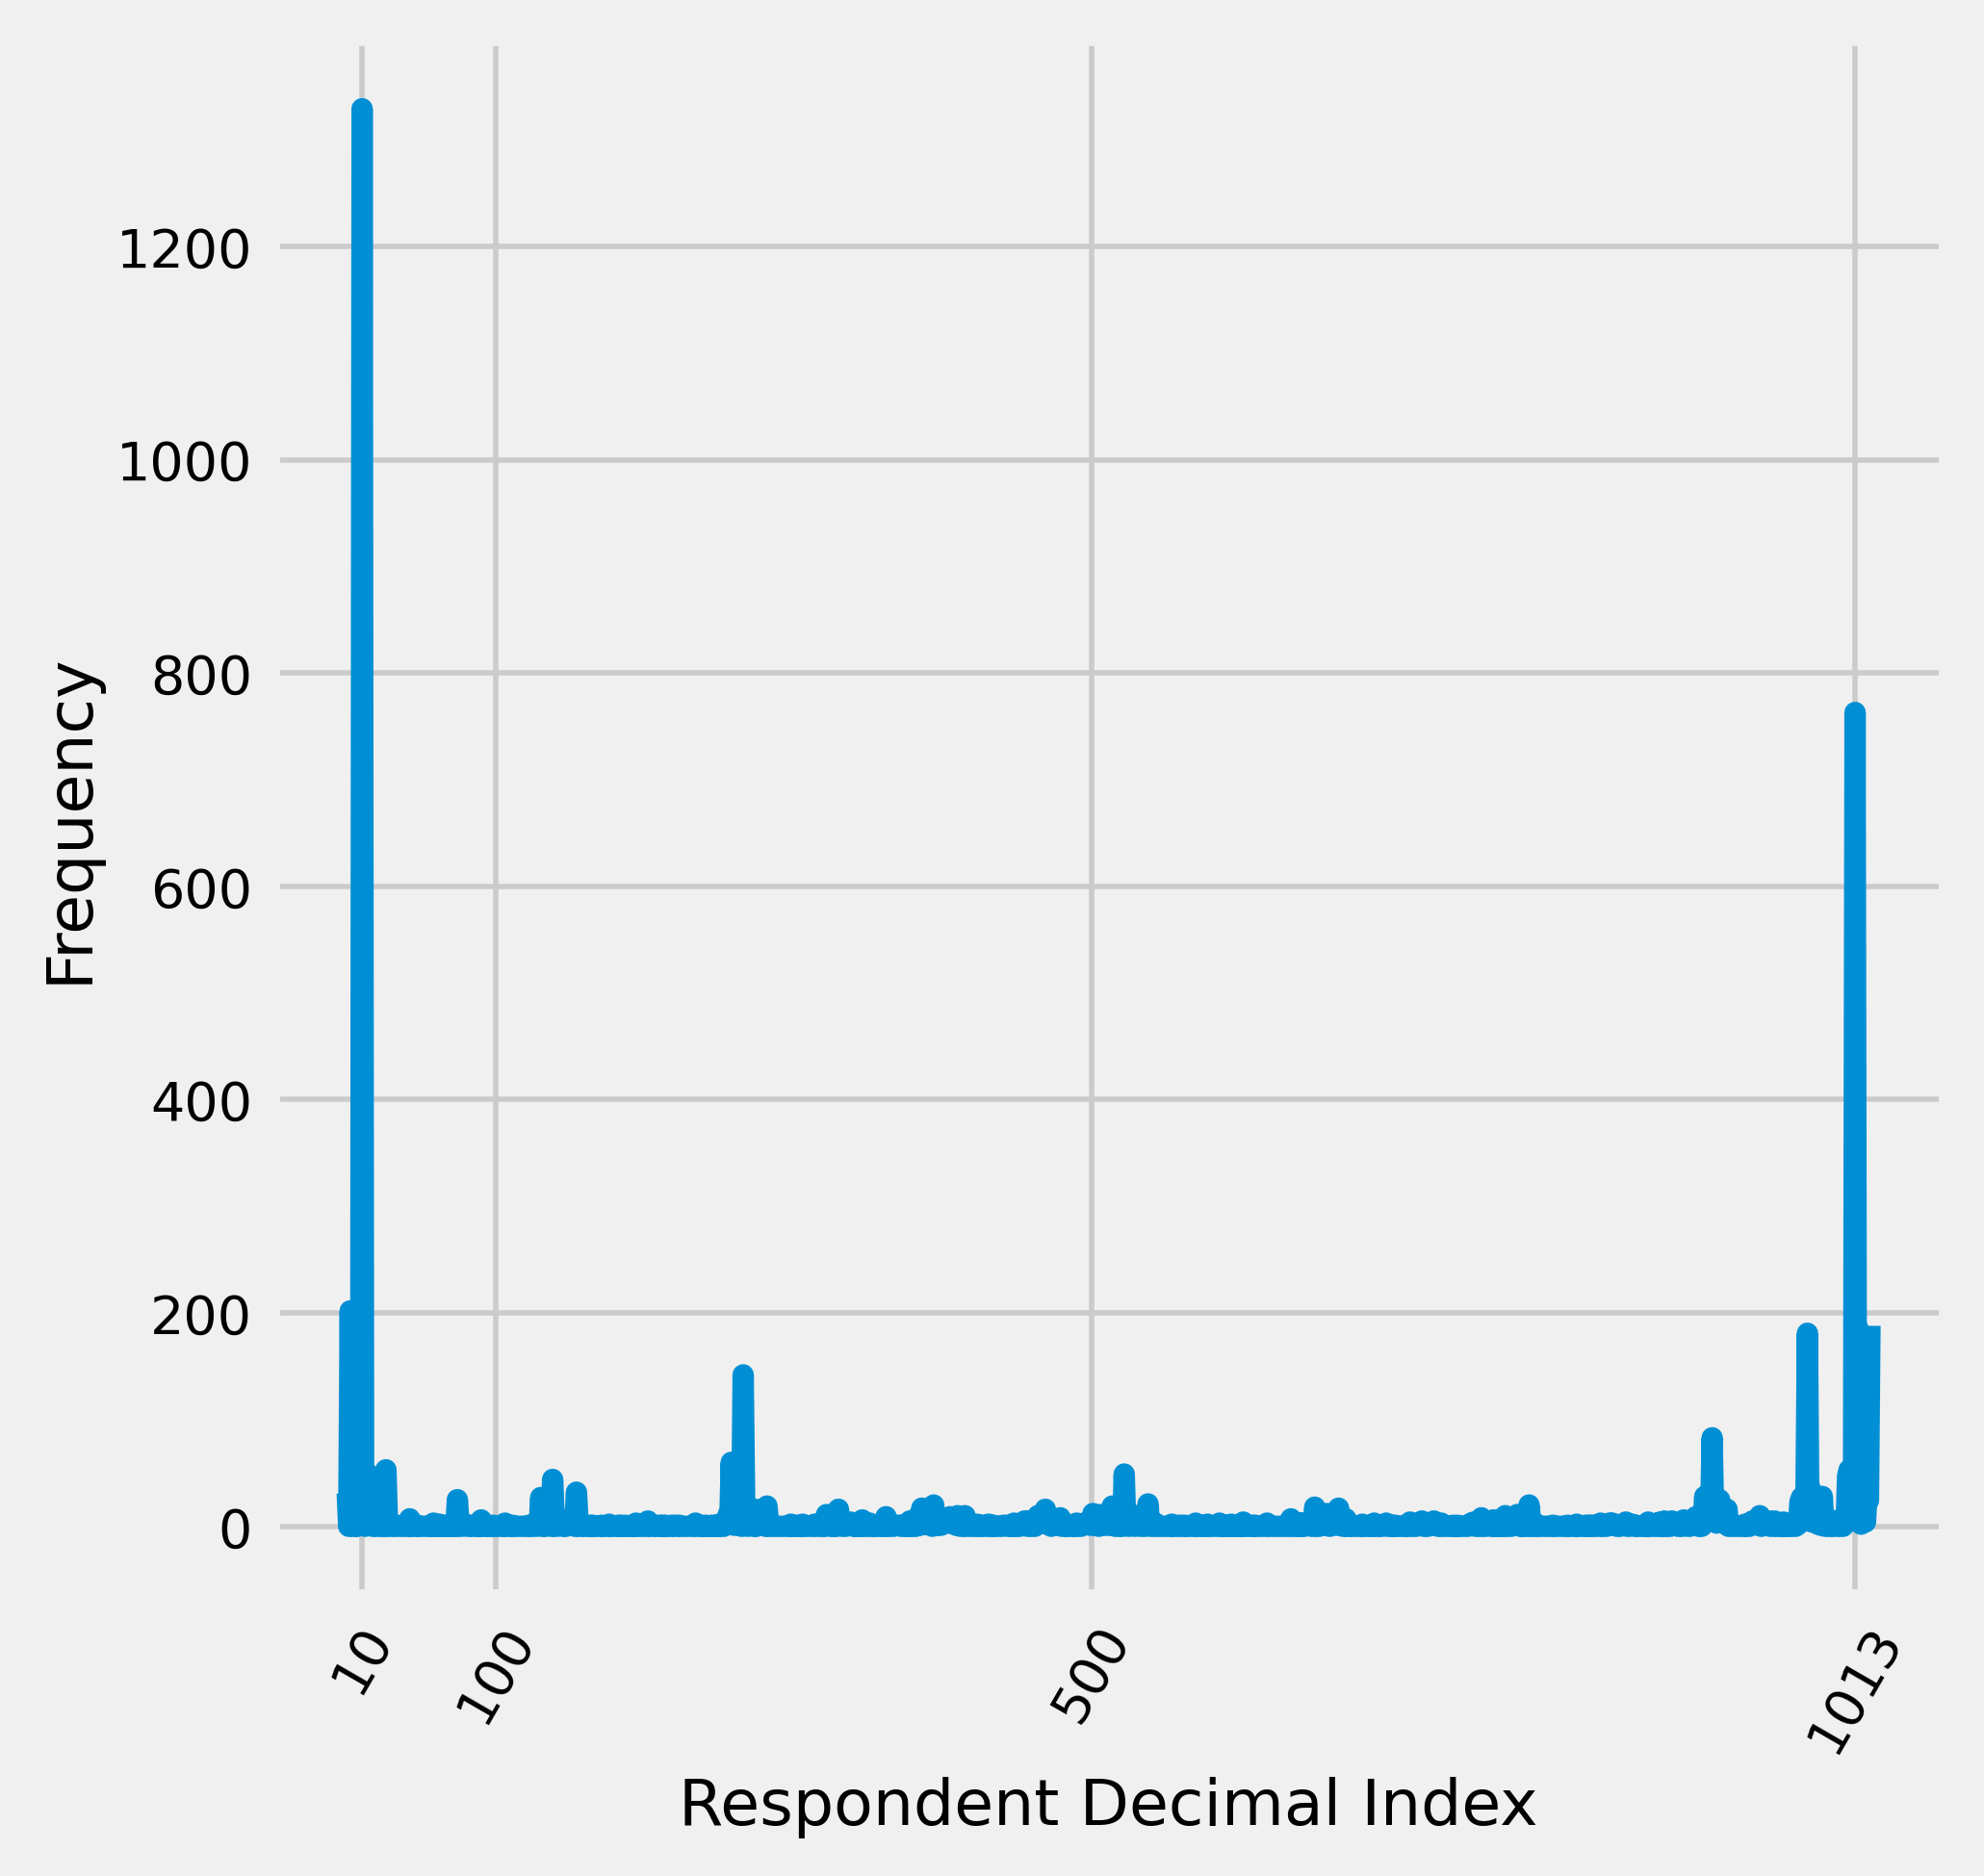
\includegraphics[width=0.4\textwidth,height=0.3\textwidth]{Fig_Gibbs_RealData.png}}
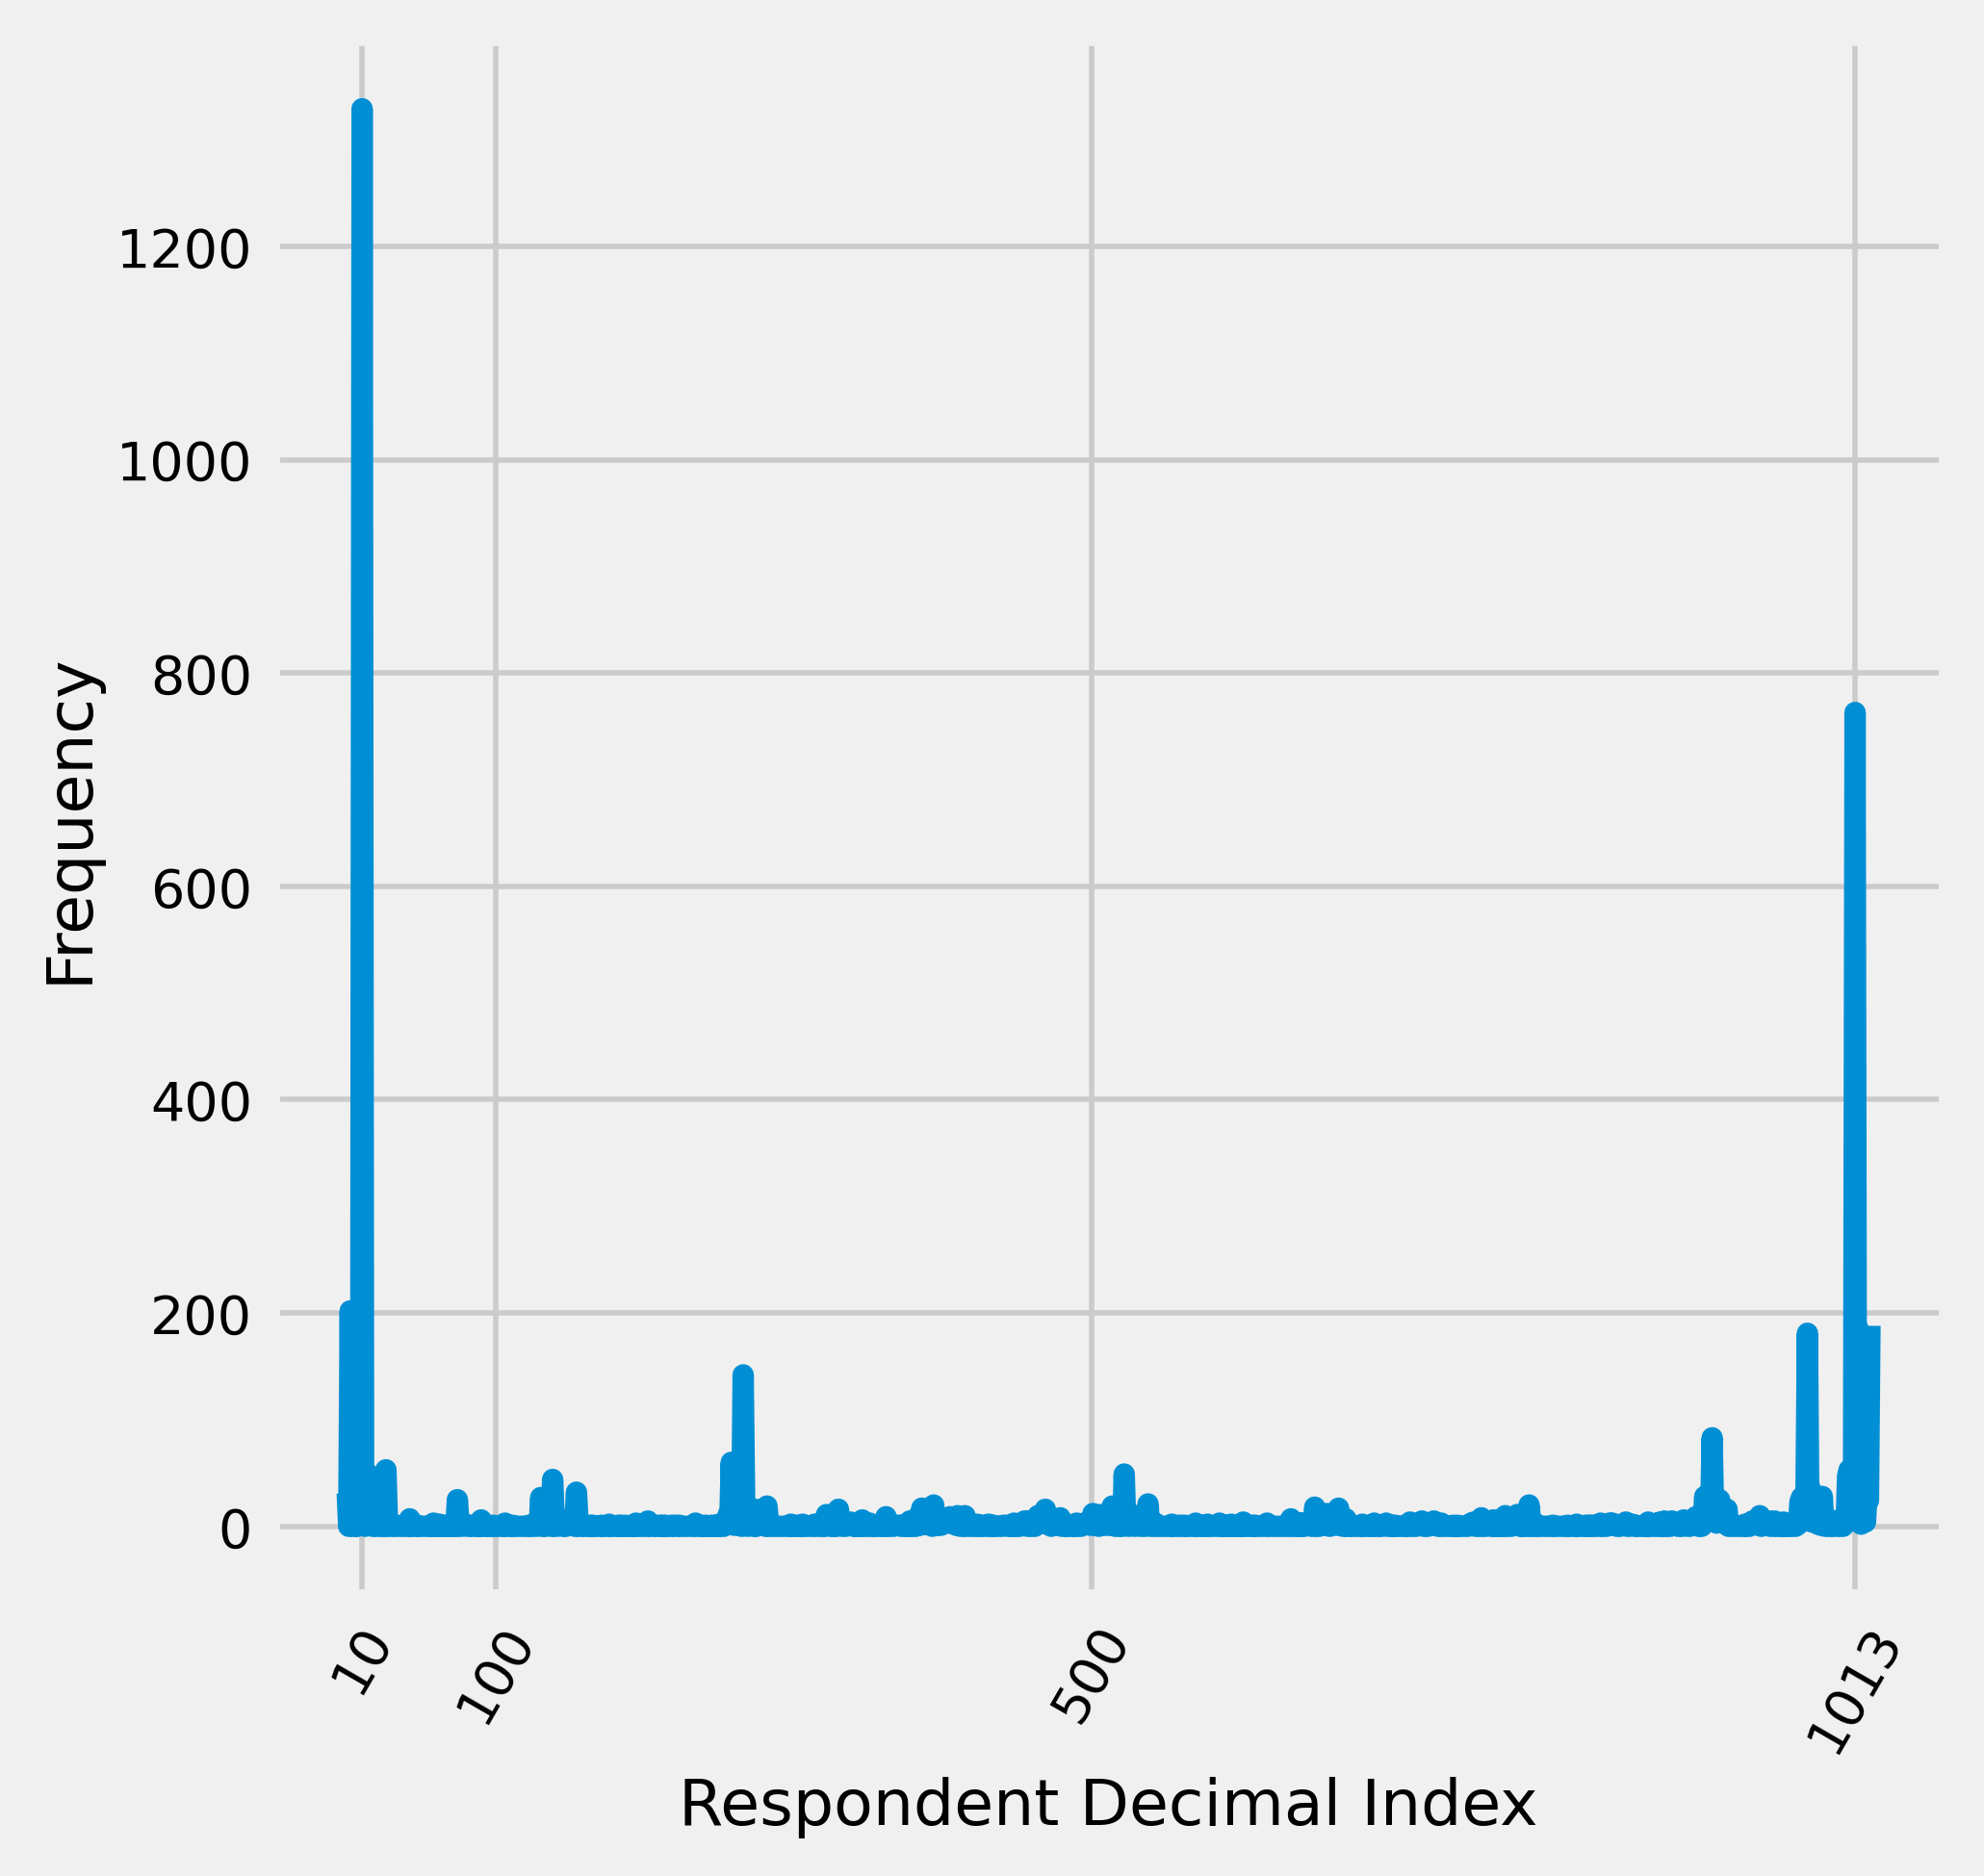
\includegraphics[width=0.4\textwidth,height=0.3\textwidth]{Fig_Gibbs_RealData.png}
\end{center}
\caption{Distribution of responses in the American National Election Survey, 2012. These data were learned by the CAN and ACT-R models.} 
\label{RealDataGibbs-figure}
\end{figure}

It is clear that the data have two prominent response patterns, pattern 10 (freq. of 1329 or 23\%) and pattern 1013 (freq. of 763 or 13\%).  Pattern 10 (0000001010) endorses only two beliefs about Barack Obama: "Makes you feel angry": \textbf{Ang, 7} and "Makes you feel afraid": \textbf{Afr, 9} (these are the only two negative attributes of Barack Obama). Pattern 1013 is the logical compliment to pattern 10 (1111110101); this pattern endorses all of the positive attributes of Barack Obama in the survey item set. 

\subsection{Study 1: Effect of Noise on Retrieval}
The next step in our work was to understand and compare the operating characteristics of the CAN and ACT-R attitude models.   To this end, we studied non-cued retrievals of both systems. Figure~\ref{numbendstates-figure} shows the number of unique retrieval patterns by noise level.  



For both attitude models (CAN and ACT-R) we see a marked increase in the number of unique retrieval patterns as noise is increased.  A key difference between the two models is that the CAN model exhibits more of a step-like function; it has little change in the number of retrieval patterns until the noise value reaches 1.  Some detail is provided in Table~\ref{can-endstate-table}.  Here we see that directly before the sharp increase in number of retrieval patterns (at CAN noise level = 0.5), 92 of the 100 retrieval attempts were either retrieval pattern 10 or 1013.  In Figure \ref{NoiseGibbs-figure}, in the second row, we show the retrieval pattern distributions for four noise levels for the CAN model. Notice that noise level 1 (panel C*), compared to 0.5 (panel B*), exhibits a much broader distribution of retrieval patterns.  In short, the retrieval output of the CAN model is very stable prior to noise value of 1 after which it devolves into a much less systematic retrieval regime.     
\begin{figure}[H]
\begin{center}
%\fbox{CoGNiTiVe ScIeNcE}
%\fbox{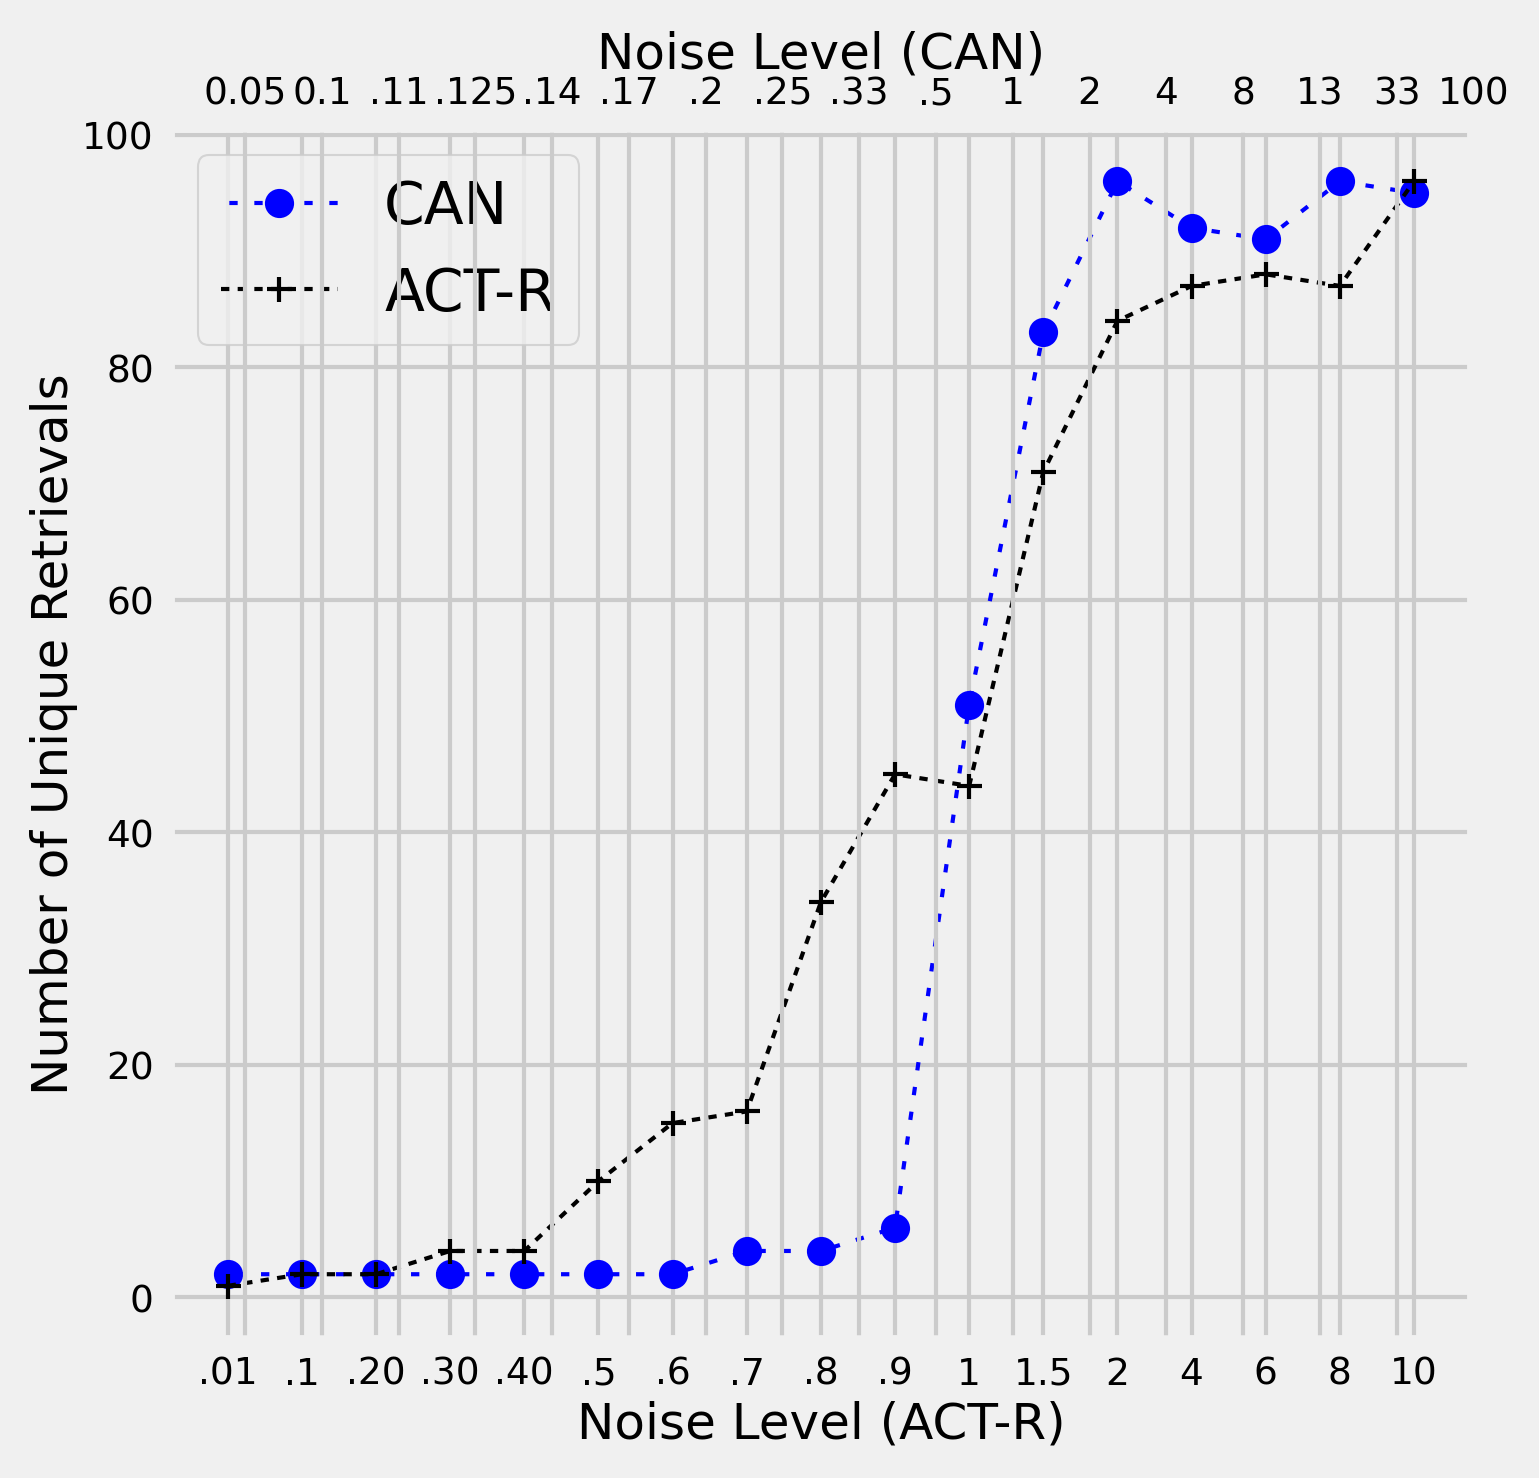
\includegraphics[width=0.4\textwidth]{Num_Endstates_CAN-IBL.png}}
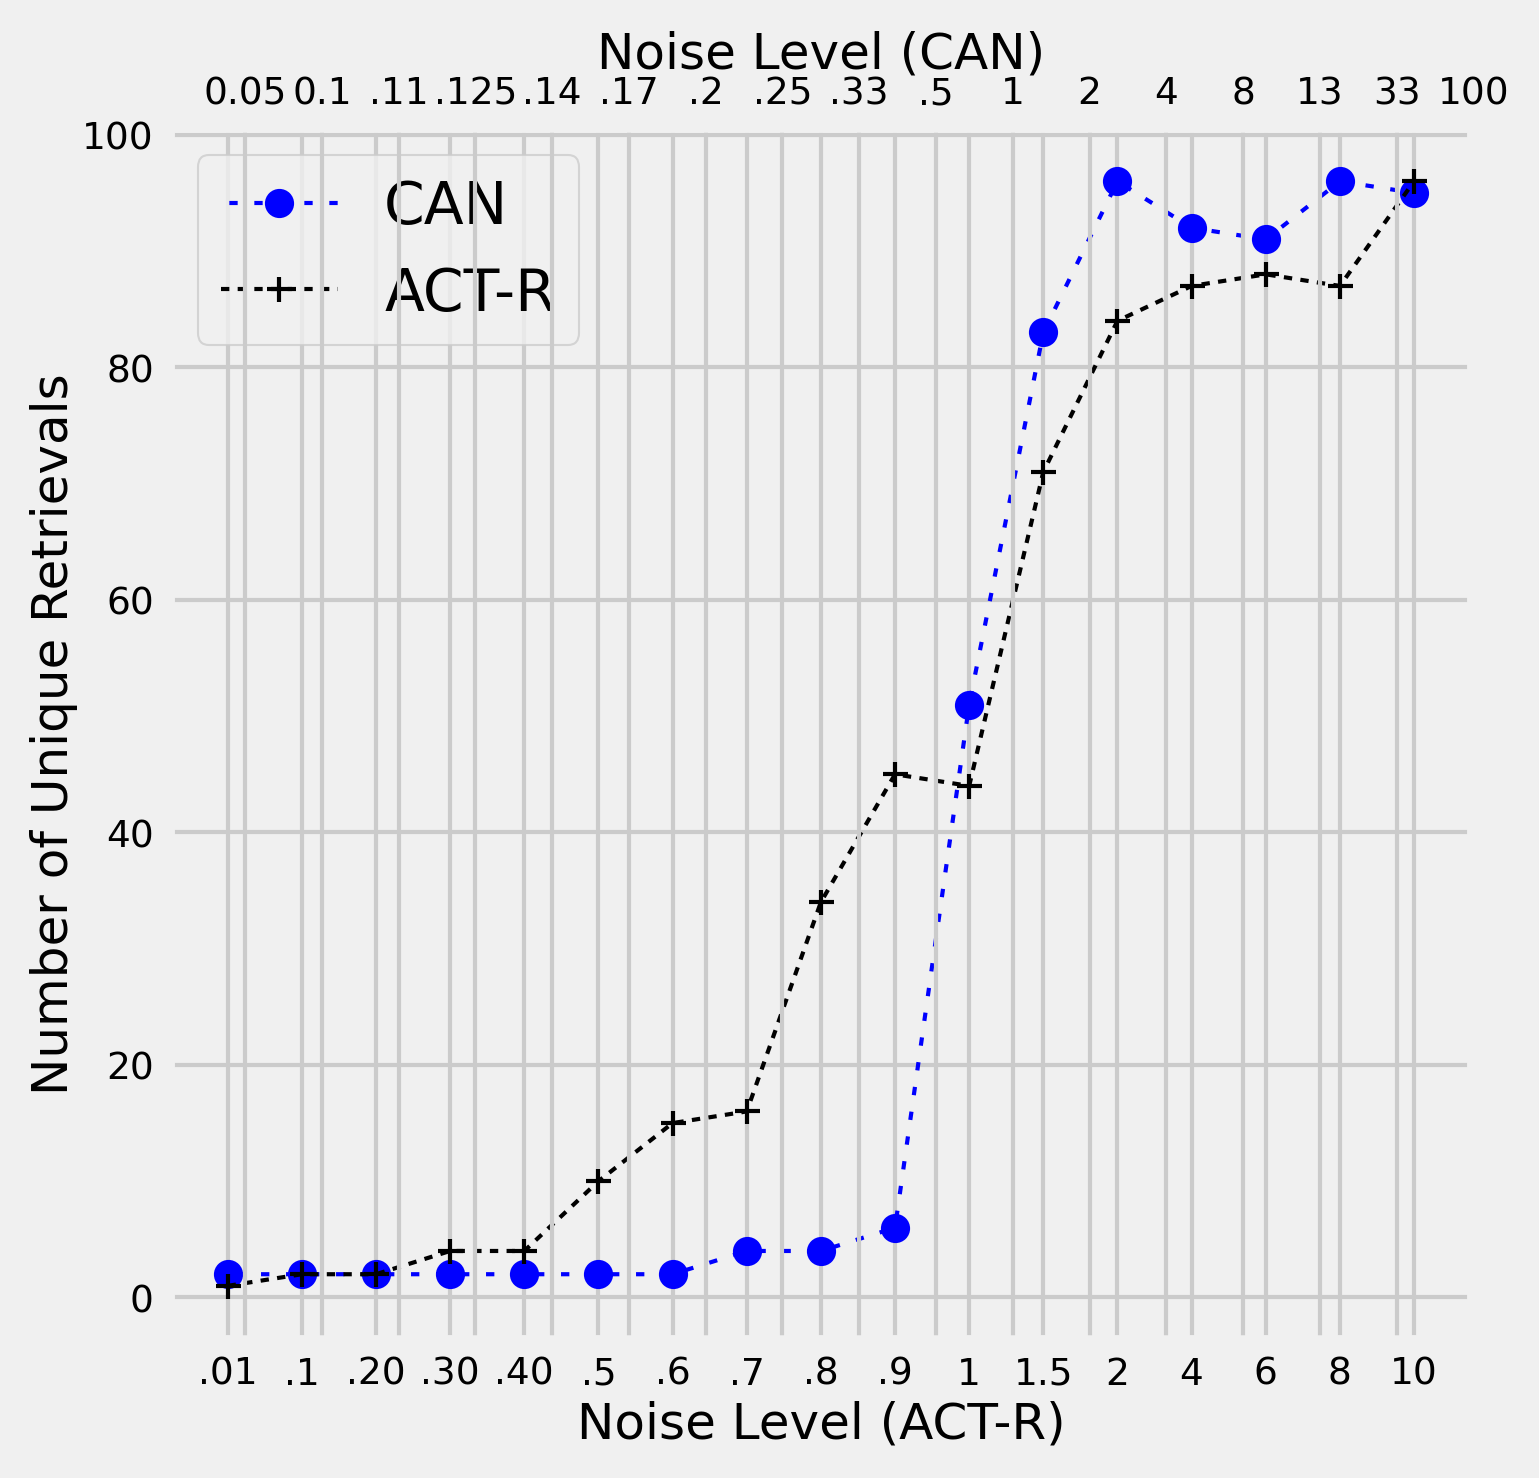
\includegraphics[width=0.4\textwidth]{Num_Endstates_CAN-IBL.png}
\end{center}
\caption{Number of unique retrieval patterns in Study 1 by model type over noise level.} 
\label{numbendstates-figure}
\end{figure}

\begin{table}[H]
\begin{center} 
\caption{Retrieval Distributions for CAN} 
\label{can-endstate-table} 
\vskip 0.12in
\begin{tabular}{llll} 
\hline
Noise  & Freq.  &  Retrievals & Dec. Retr.\\
\hline
0.11    & 81  &    1111110101 & 1013 \\
& 18    & 0000001010 & 10 \\
\hline
0.25    & 74  &    1111110101 & 1013 \\
& 23    & 0000001010 & 10 \\
     & 1 & 1111010101 & 981 \\
     & 1 & 1111111111 & 1023\\
\hline
0.50    & 59  &    1111110101 & 1013 \\
& 33    & 0000001010 & 10 \\
             & 3 & 0000000010 & 2 \\
        & $<3$ & 1111110000 & 1008\\
        & $<3$ & 1111110111 & 1015\\
        & $<3$ & 1111111111 & 1023\\
\hline
\end{tabular} 
\end{center} 
\end{table}

The ACT-R model shows more graded increase in the number of unique retrieval patterns. Yet, in Table \ref{ibl-endstate-table} we see that even as the number of retrieval patterns starts to increase--compare ACT-R noise of 0.4 to 0.5--the two dominant retrieval patterns were represented by 87 of the 100 retrievals for noise level 0.5.  In Figure \ref{NoiseGibbs-figure}, in the first row, we show the retrieval pattern distributions for four noise levels for the ACT-R model. Notice that noise level 0.9 (panel C), compared to 0.5 (panel B), exhibits a much broader distribution of retrieval patterns. 

Figure \ref{NoiseGibbs-figure} offers three other comparisons between the two models. First, and most striking, is that the distributions of the two models under low noise levels are near complements. Second, we see clearly that the ACT-R model matches the frequency pattern observed in the survey data (see Figure \ref{RealDataGibbs-figure}) while the CAN model does not; yet both models, with low levels of noise capture the two most frequent patterns found in the data, 10 and 1013. Third, both models show some degree of maintaining their retrieval distribution even under noisy conditions. In panels C and C* we still see a rank similarity to panels A and A* respectively given significant noise. In other words, the first order feature of the learned retrieval distribution is somewhat robust to a significant degree of noise in both systems.

\begin{table}%[H]
\begin{center} 
\caption{Retrieval Distributions for ACT-R} 
\label{ibl-endstate-table} 
%\vskip 0.12in
\begin{tabular}{llll} 
\hline
Noise  & Freq.  &  Retrievals & Dec. Retr.\\
\hline
0.2 & 81    & 0000001010 & 10 \\
    & 18  &    1111110101 & 1013 \\
\hline

0.4 &    75    & 0000001010 & 10 \\
        & 22  &    1111110101 & 1013 \\
     & 1 & 1111110111 & 1015 \\
     & 1 & 0000000010 & 2\\
\hline
0.5 &    56    & 0000001010 & 10\\
        & 31  &    1111110101 & 1013\\
             & 4 & 0000000010 & 2 \\
        & $<3$ & 0000001000 & 8 \\
        & $<3$ & 0100000010 & 258\\
        & $<3$ & 1110010101 & 917\\
        & $<3$ & 1111110010 & 1010\\
        & $<3$ & 1111110111 & 1015\\
        & $<3$ & 1111111010 & 1018\\
        & $<3$ & 1111111111 & 1023\\
\hline
\end{tabular} 
\end{center} 
\end{table}
%
\begin{figure}%[H]
\begin{center}
%\fbox{CoGNiTiVe ScIeNcE}
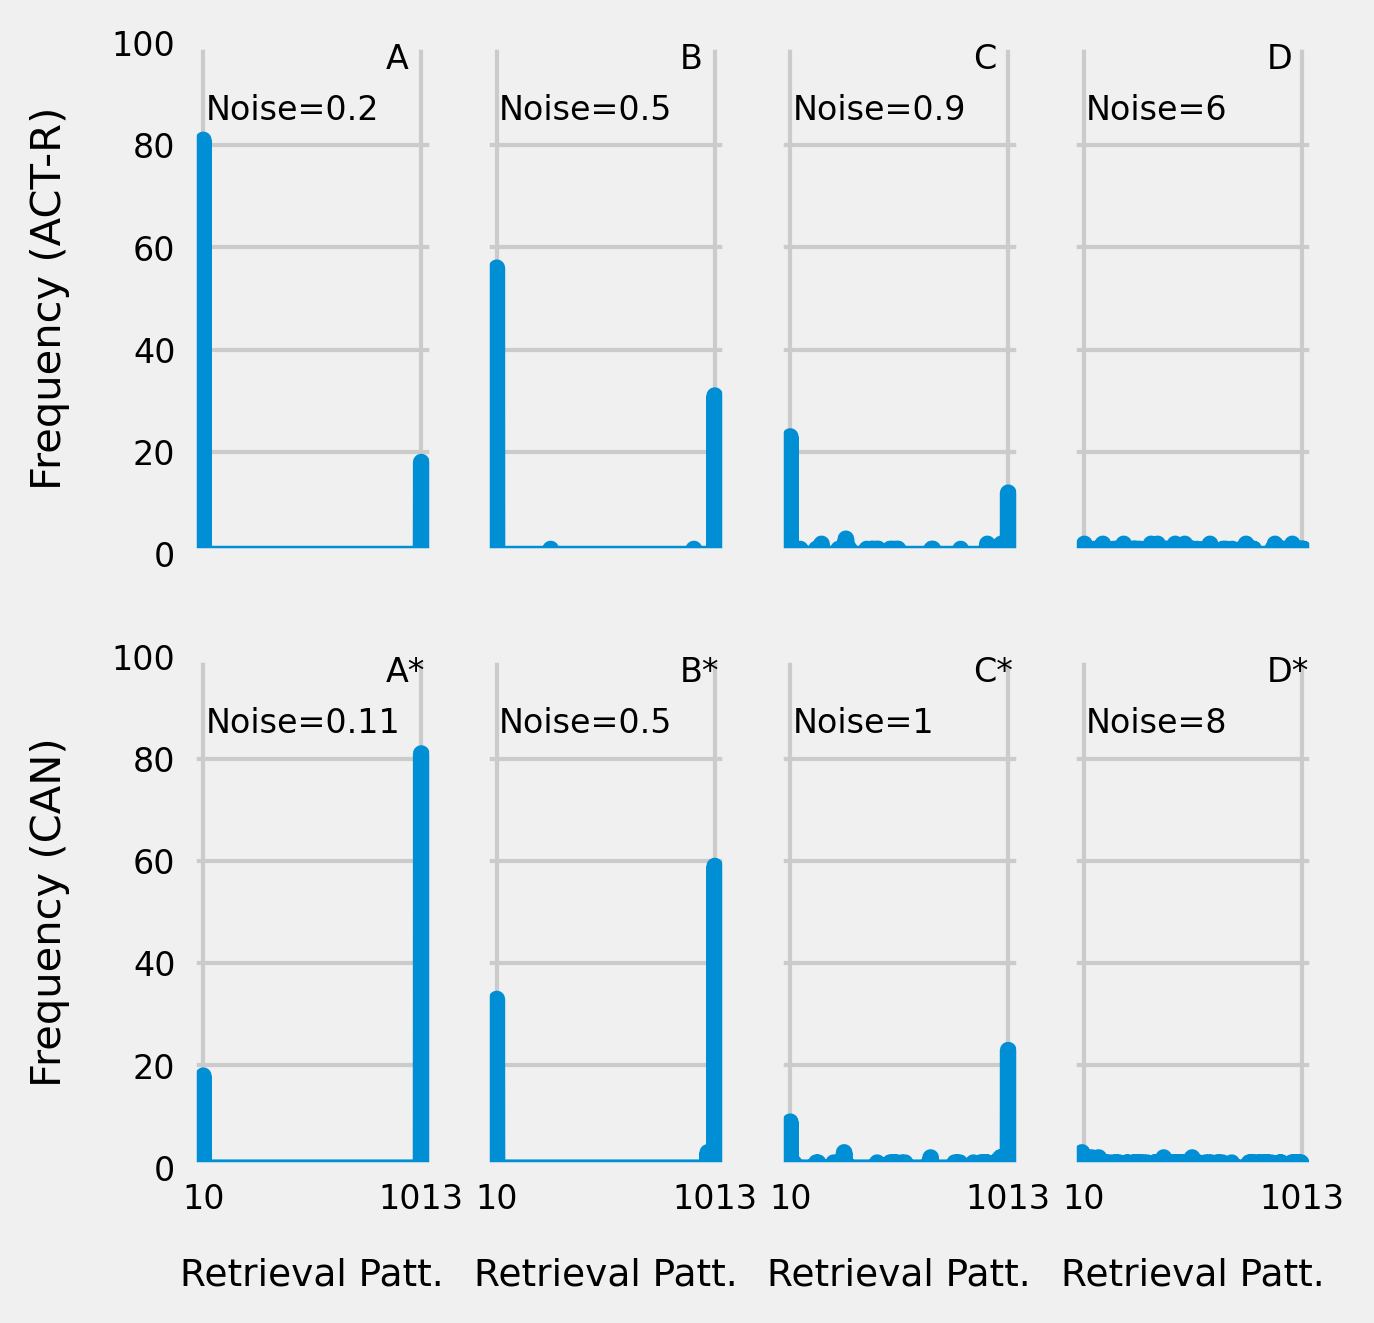
\includegraphics[width=0.4\textwidth,height=0.3\textwidth]{CAN_Gibbs_2X4.png}
\end{center}
\caption{The distribution of retrieval patterns by model for varying levels of noise.} 
\label{NoiseGibbs-figure}
\end{figure}
In sum, Study 1 shows similarities across the two models.  At lower levels of noise, both models retrieve the two dominant response patterns found in the data.  Although the CAN model shows a steeper noise profile, the rank order distributions are captured by both models up to a degree even with significant noise.  However, we do see a very marked difference in the relation to the survey data response distribution and the model retrieval pattern distributions.  The ACT-R model captures it well while the CAN model provides more like a complement to the survey data distribution. Specifically, at noise level 0.5 for both models, the ACT-R model roughly reproduces the relative ratio of the two most popular patterns in the data set (10 and 1013, respectively), while the CAN model also roughly reproduces that ratio but inverted. We will address this latter point in the Conclusion section.

\subsection{Study 2: Cued Retrieval}
The next step was to compare the CAN and ACT-R attitude models when cued.  Figure~\ref{CuedWass-figure} shows the Wasserstein distance between the distribution of retrieval patterns for each cued condition and a baseline non-cued distribution of retrieval patterns (generated in Study 1; for both CAN and ACT-R we used noise=0.5). This provides a measure of the difference in the low noise, non-cued behavior of the model compared to the cue for each condition (with the same level of noise).  The first-order results are clear.  Both models show a similar pattern across retrieval cues; both showed clear dips for the cues \textbf{Ang} and \textbf{Afr} (the only negative beliefs in the item set).  Further, the ACT-R model was clearly higher in Wasserstein distance across the board.  

\begin{figure}[H]
\begin{center}
%\fbox{CoGNiTiVe ScIeNcE}
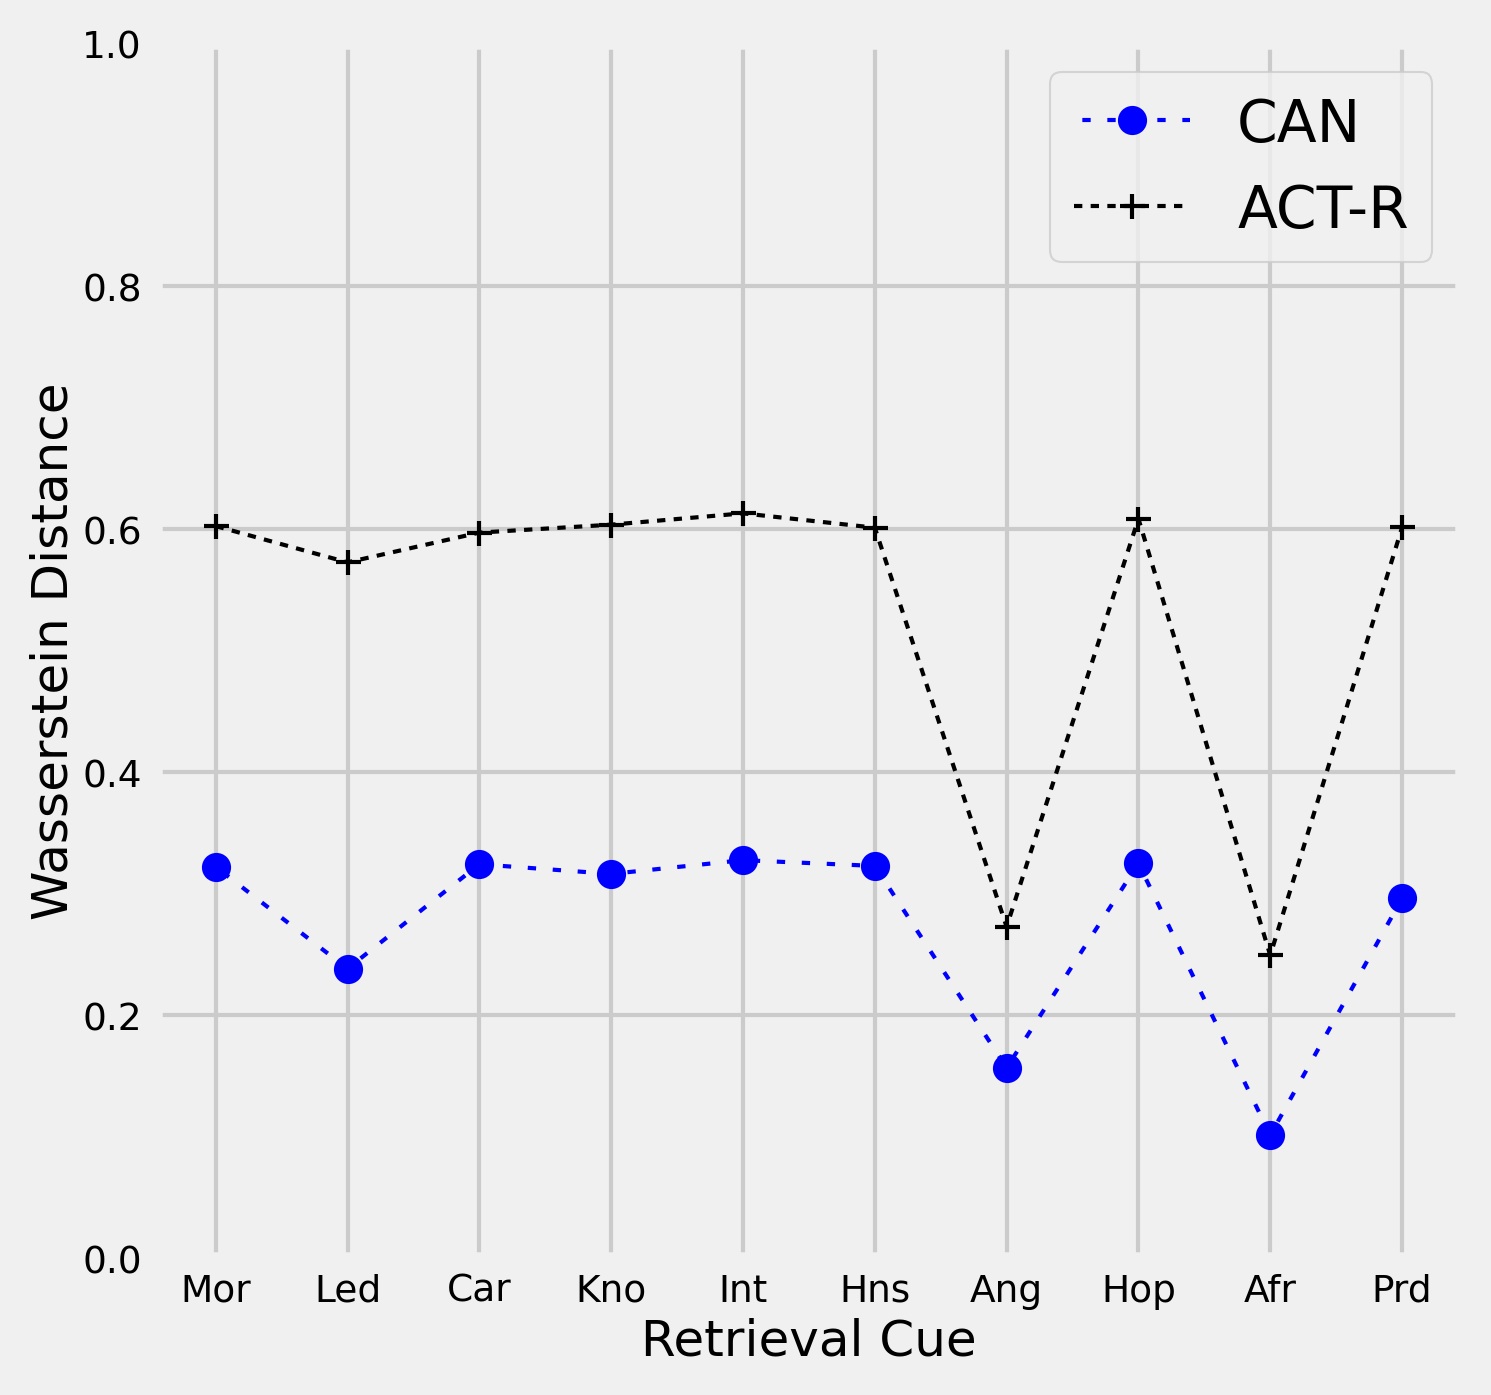
\includegraphics[width=0.4\textwidth,height=0.3\textwidth]{Cued_WASS_CAN-IBL.png}
\end{center}
\caption{Wasserstein distance between low noise, non-cued conditions (Study 1) and low noise cued conditions (Study 2). } 
\label{CuedWass-figure}
\end{figure}

Figures \ref{can-gibbs-cued-figure} and \ref{ibl-gibbs-cued-figure} shed some light on these patterns.  It is useful to characterize each  cued distribution in reference to the referent non-cued conditions in Study 1 (the latter are shown in Figure \ref{NoiseGibbs-figure} in panels B and B*).  For the CAN model, we see that the Wasserstein differences shown in Figure \ref{CuedWass-figure} were driven by the same distribution pattern such that virtually all retrieval patterns were pattern 1013, excepting the two, negatively valenced cued conditions \textbf{Ang} and \textbf{Afr}. This behavior makes sense given that these eight cues were all present in pattern 1013 and pattern 1013 was very frequent given non-cued retrieval for the CAN model. The remaining cue conditions \textbf{Ang} and \textbf{Afr}, however, showed a mixed distribution, largely across retrieval patterns 10 and 1013.  This behavior illustrates a difficulty with the system to operate well when these two negatively valenced beliefs were cued.  

For the ACT-R model, a somewhat different story emerged.  For the eight positively valenced cues, the behavior was similar to the CAN model.  Notice that this runs counter to the ACT-R non-cued distribution and the frequencies in the survey data (see Figure \ref{RealDataGibbs-figure}).  Thus, the ACT-R model provided a reasonable retrieval despite the frequency demands of retrieval pattern 10.  This provides a way to interpret the larger Wasserstein distances for ACT-R in Figure \ref{CuedWass-figure} as indicative of accurate retrieval.  For the two negatively valenced cues \textbf{Ang} and \textbf{Afr} we see a marked difference from the CAN model.  Most of the ACT-R retrievals for these two cues are for pattern 10, a very reasonable response.  

In sum, the behavior for the CAN model was driven largely by its baseline, non-cued retrieval tendencies.  This seemed to work in its favor but only for the eight cues of positive valence.  The ACT-R model, on the other hand, responded equally well to all cues and did so in the face of the frequency demands of the learning environment.  Thus, the ACT-R attitude model showed more appropriate behavior in respect to its cues compared to the CAN model. 
\begin{figure}[H]
\begin{center}
%\fbox{CoGNiTiVe ScIeNcE}
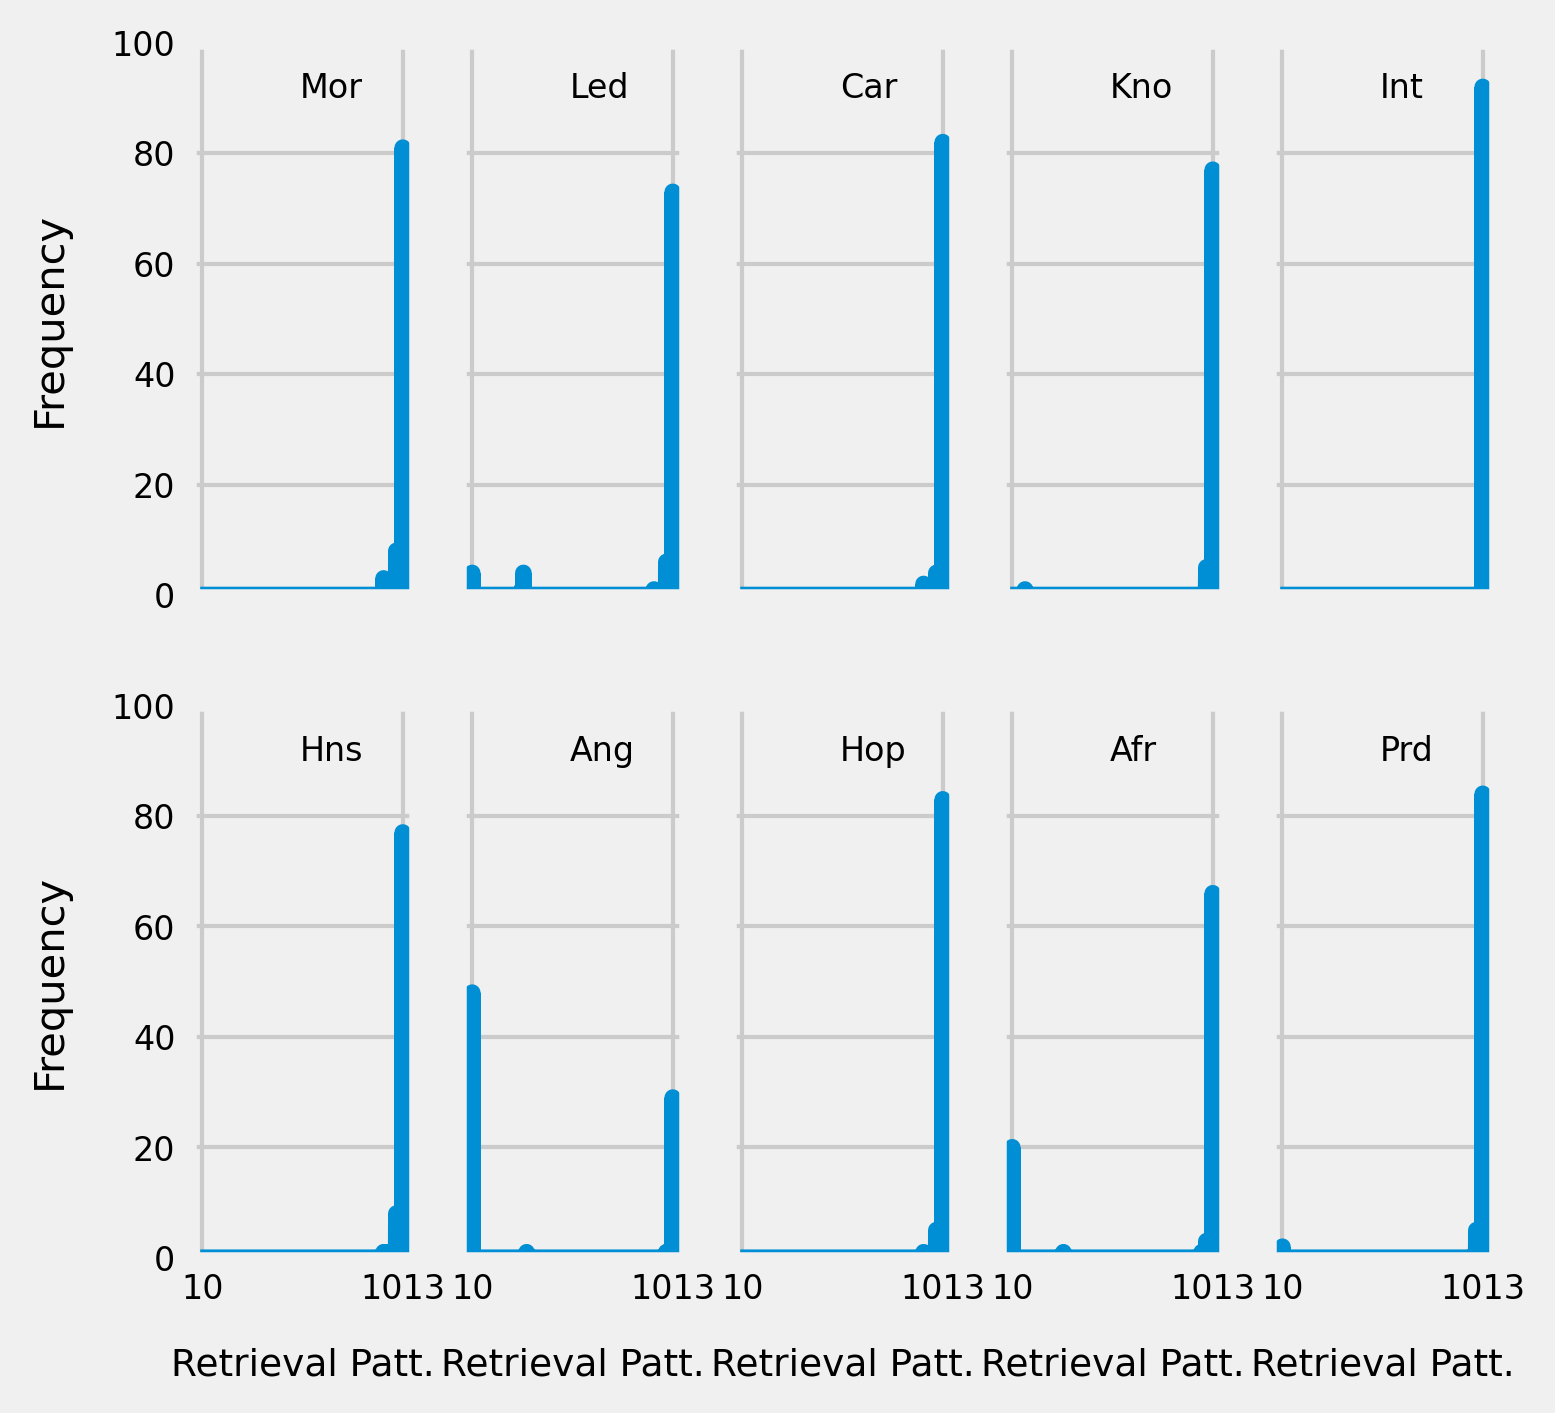
\includegraphics[width=0.4\textwidth,height=0.3\textwidth]{CAN_Gibbs_Cued_2X5.png}
\end{center}
\caption{The distribution of retrieval patterns by cue for the CAN model.} 
\label{can-gibbs-cued-figure}
\end{figure}

\begin{figure}[H]
\begin{center}
%\fbox{CoGNiTiVe ScIeNcE}
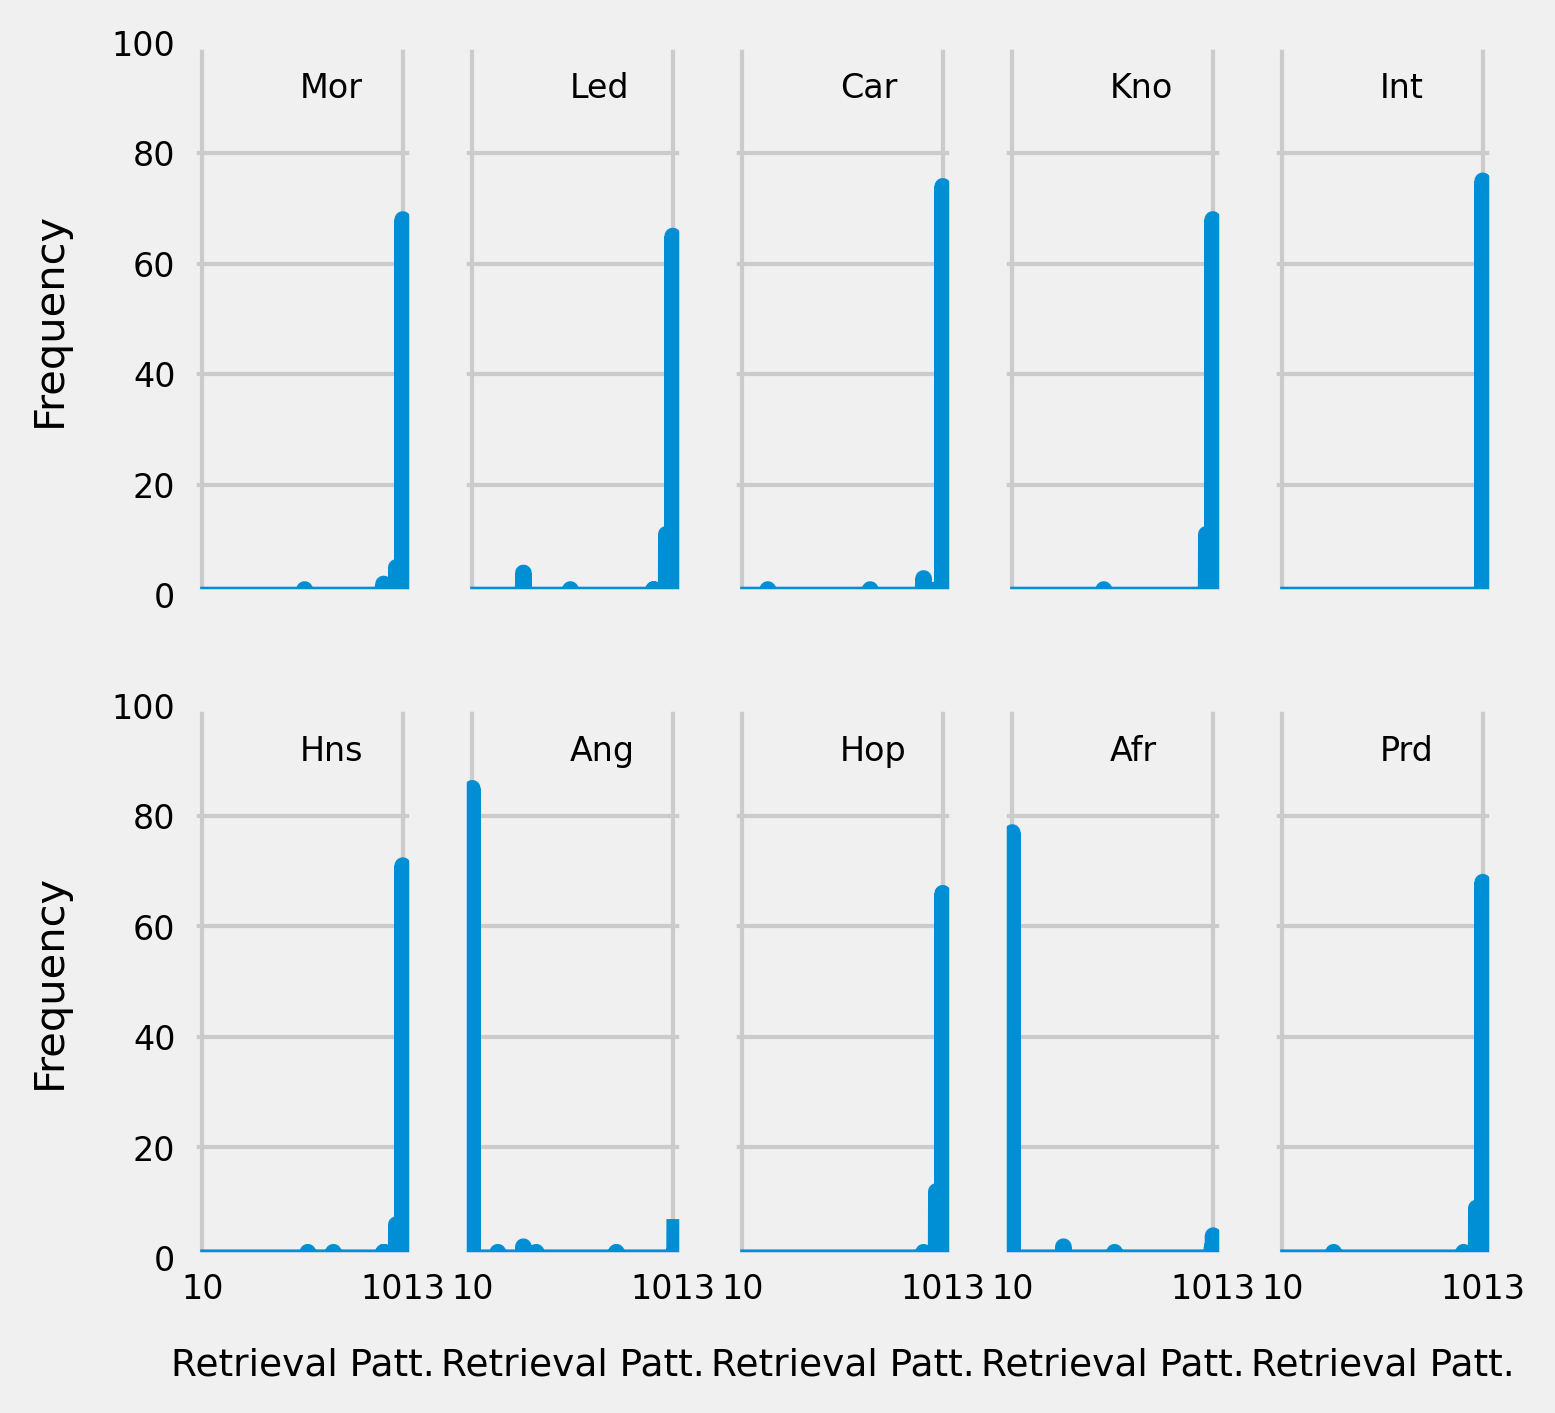
\includegraphics[width=0.4\textwidth,height=0.3\textwidth]{IBL_Gibbs_Cued_2X5.png}
\end{center}
\caption{The distribution of retrieval patterns by cue for the ACT-R model.} 
\label{ibl-gibbs-cued-figure}
\end{figure}


\section{Conclusions}\label{conclusion}
In conclusion, the CAN and ACT-R attitude models showed marked differences.  First, when not cued, both models exhibited retrieval that captured the two most frequent response patterns in the survey data (patterns 10 and 1013) but the CAN model generated retrieval frequencies that were nearly complimentary to the ACT-R model and that were not aligned with the frequencies found in the survey data.  Second, under cue conditions, the ACT-R model was more adaptive to the cues and was able to override the frequencies in the survey data.  The CAN model did not exhibit such adaptability.

The conceptual language of the CAN model literature has not been in terms of retrievals, but in terms of changes in attractor states under perturbation (e.g., fix a value of $\tau_i$ as we did for Study 2) or differences in attractor states given systematic differences in graph topology (e.g., larger values of the weights $w_{ij}$s or a more dense set of weights $w_{ij}$s) \citep{dalege2016,DalegeMaas2017,DalegevanderMaas2020}. Although there is no technical difference between retrieval or perturbation in the CAN model, the language of perturbation captures a different semantic and a different emphasis.  The CAN model is an outgrowth of the psychological networks literature that originated, in large part, in clinical psychology \citep[see][]{Bringmann2018, Bringmann2021, bringmann2019centrality, WichersWigman2015, cramer2016major, burger2020bridging, haslbeck2021modeling}.  This literature is primarily concerned with the relation between graph properties and how they can predict changes in the graph states. Thus, the language of perturbation is apt.  

However, we find the extension of the perturbation semantic to attitudinal memory models to be misguided (without further revision of the CAN model).  Retrieval is in reference to the purpose of the system.  In the studies above, we assumed that the survey data was a proxy for a set of social exposures and the goal of the model was to learn from its social contexts.  This is not the typical emphasis in the CAN model literature. Yet, understanding the effects of perturbation on a model without reference to what was learned will not push the CAN model towards a useful, applicable model of attitude formation.  

The resulting graph generated via the CAN learning procedure (see Design section) exhibits many excitatory positive weights with a small set of inhibitory negative weights. Thus, the lack of adaptability to cues shown in Study 2 was not surprising. The system captures correlations but when used in a dynamic associative memory network, the cuing did not work well in part because the model was not designed with sensible cuing in mind. The ACT-R model, by virtue of its grounding in a cognitive architecture and its underlying rational analysis of cognition (\cite{anderson1990}), inherited adaptive and reasonable cuing behavior.  Our final assessment is that, if the CAN model is to be viable, then it should move beyond an analysis of its network and think towards a sensible cuing system, in the name of external validity. 

On a more general note we offer the following reflection.  Despite their superficial differences, commonalities between ACT-R declarative memory and Hopfield-like networks have been previously exploited. Most notably, Hopfield networks were used to implement declarative memory in the connectionist implementation of ACT-R, ACT-RN (\cite{lebiere1993connectionist}). Noteworthy aspects include using separate Hopfield networks for each type of chunks, reflecting different number of slots as well as distinct semantics, and adding winner-take-all dynamics for chunk identifiers to prevent merging of chunks with similar distributed representations.  The recognition of this duality between cognitive architectures and connectionist models led to a direct comparison between ACT-R and PDP models according to a set of criteria for unified theories of cognition (\cite{anderson2003newell}). While the two paradigms were judged to have distinct strengths and weaknesses, they were also found to have commonalities for criteria relevant to attitude formation such as learning and adaptive behavior. Thus, when modeling attitudes, such consideration may inform future work including a potential unification of the two modeling frameworks.


\printbibliography 


\end{document}
